\documentclass[journal,12pt,twocolumn]{IEEEtran}

\usepackage{setspace}
\usepackage{gensymb}
\singlespacing
\usepackage[cmex10]{amsmath}

\usepackage{amsthm}

\usepackage{mathrsfs}
\usepackage{txfonts}
\usepackage{stfloats}
\usepackage{bm}
\usepackage{cite}
\usepackage{cases}
\usepackage{subfig}
\usepackage{tabularx}
\usepackage{longtable}
\usepackage{multirow}
\usepackage{blkarray}
\usepackage{enumitem}
\usepackage{mathtools}
\usepackage{steinmetz}
\usepackage{tikz}
\usepackage{circuitikz}
\usepackage{verbatim}
\usepackage{tfrupee}
\usepackage[breaklinks=true]{hyperref}
\usepackage{graphicx}
\usepackage{tkz-euclide}
\usetikzlibrary{automata, positioning}
\usetikzlibrary{calc,math}
\usepackage{listings}
    \usepackage{color}                                            %%
    \usepackage{array}                                            %%
    \usepackage{longtable}                                        %%
    \usepackage{calc}                                             %%
    \usepackage{multirow}                                         %%
    \usepackage{hhline}                                           %%
    \usepackage{ifthen}                                           %%
    \usepackage{lscape}     
\usepackage{multicol}
\usepackage{chngcntr}

\DeclareMathOperator*{\Res}{Res}

\renewcommand\thesection{\arabic{section}}
\renewcommand\thesubsection{\thesection.\arabic{subsection}}
\renewcommand\thesubsubsection{\thesubsection.\arabic{subsubsection}}

\renewcommand\thesectiondis{\arabic{section}}
\renewcommand\thesubsectiondis{\thesectiondis.\arabic{subsection}}
\renewcommand\thesubsubsectiondis{\thesubsectiondis.\arabic{subsubsection}}


\hyphenation{op-tical net-works semi-conduc-tor}
\def\inputGnumericTable{}                                 %%

\lstset{
%language=C,
frame=single, 
breaklines=true,
columns=fullflexible
}
\begin{document}


\newtheorem{theorem}{Theorem}[section]
\newtheorem{problem}{Problem}
\newtheorem{proposition}{Proposition}[section]
\newtheorem{lemma}{Lemma}[section]
\newtheorem{corollary}[theorem]{Corollary}
\newtheorem{example}{Example}[section]
\newtheorem{definition}[problem]{Definition}

\newcommand{\BEQA}{\begin{eqnarray}}
\newcommand{\EEQA}{\end{eqnarray}}
\newcommand{\define}{\stackrel{\triangle}{=}}
\bibliographystyle{IEEEtran}
\raggedbottom
\setlength{\parindent}{0pt}
\providecommand{\mbf}{\mathbf}
\providecommand{\pr}[1]{\ensuremath{\Pr\left(#1\right)}}
\providecommand{\qfunc}[1]{\ensuremath{Q\left(#1\right)}}
\providecommand{\sbrak}[1]{\ensuremath{{}\left[#1\right]}}
\providecommand{\lsbrak}[1]{\ensuremath{{}\left[#1\right.}}
\providecommand{\rsbrak}[1]{\ensuremath{{}\left.#1\right]}}
\providecommand{\brak}[1]{\ensuremath{\left(#1\right)}}
\providecommand{\lbrak}[1]{\ensuremath{\left(#1\right.}}
\providecommand{\rbrak}[1]{\ensuremath{\left.#1\right)}}
\providecommand{\cbrak}[1]{\ensuremath{\left\{#1\right\}}}
\providecommand{\lcbrak}[1]{\ensuremath{\left\{#1\right.}}
\providecommand{\rcbrak}[1]{\ensuremath{\left.#1\right\}}}
\theoremstyle{remark}
\newtheorem{rem}{Remark}
\newcommand{\sgn}{\mathop{\mathrm{sgn}}}
\providecommand{\abs}[1]{\left\vert#1\right\vert}
\providecommand{\res}[1]{\Res\displaylimits_{#1}} 
\providecommand{\norm}[1]{\left\lVert#1\right\rVert}
%\providecommand{\norm}[1]{\lVert#1\rVert}
\providecommand{\mtx}[1]{\mathbf{#1}}
\providecommand{\mean}[1]{E\left[ #1 \right]}
\providecommand{\fourier}{\overset{\mathcal{F}}{ \rightleftharpoons}}
%\providecommand{\hilbert}{\overset{\mathcal{H}}{ \rightleftharpoons}}
\providecommand{\system}{\overset{\mathcal{H}}{ \longleftrightarrow}}
	%\newcommand{\solution}[2]{\textbf{Solution:}{#1}}
\newcommand{\solution}{\noindent \textbf{Solution: }}
\newcommand{\cosec}{\,\text{cosec}\,}
\providecommand{\dec}[2]{\ensuremath{\overset{#1}{\underset{#2}{\gtrless}}}}
\newcommand{\myvec}[1]{\ensuremath{\begin{pmatrix}#1\end{pmatrix}}}
\newcommand{\mydet}[1]{\ensuremath{\begin{vmatrix}#1\end{vmatrix}}}
\numberwithin{equation}{subsection}
\makeatletter
\@addtoreset{figure}{problem}
\makeatother
\let\StandardTheFigure\thefigure
\let\vec\mathbf
\renewcommand{\thefigure}{\theproblem}
\def\putbox#1#2#3{\makebox[0in][l]{\makebox[#1][l]{}\raisebox{\baselineskip}[0in][0in]{\raisebox{#2}[0in][0in]{#3}}}}
     \def\rightbox#1{\makebox[0in][r]{#1}}
     \def\centbox#1{\makebox[0in]{#1}}
     \def\topbox#1{\raisebox{-\baselineskip}[0in][0in]{#1}}
     \def\midbox#1{\raisebox{-0.5\baselineskip}[0in][0in]{#1}}
\vspace{3cm}
\title{Assignment 3}
\author{Tanay Yadav - AI20BTECH11026}
\maketitle
\newpage
\bigskip
\renewcommand{\thefigure}{\theenumi}
\renewcommand{\thetable}{\theenumi}
Download the python codes from 
\begin{lstlisting}
https://github.com/tanayyadav28/Assignments/blob/main/Assignment%203/code/assignment3.py
\end{lstlisting}
%
and latex-tikz codes from 
%
\begin{lstlisting}
https://github.com/tanayyadav28/Assignments/blob/main/Assignment%203/assignment3.tex
\end{lstlisting}
\section{Problem}
(GATE EC, Q. 25) A fair coin is tossed till a head appears for the first time. The probability that the number of requried tosses is odd,is\\
\begin{enumerate}
    \item $\dfrac{1}{3}$\\
    \item $\dfrac{1}{2}$\\
    \item $\dfrac{2}{3}$\\
    \item $\dfrac{3}{4}$
\end{enumerate}
\section{Solution}
Given that the coin is tossed until a head appears on an odd toss.\\
\begin{align}
    p = \frac{1}{2}, q = \frac{1}{2}
\end{align}

 Let's define a Markov chain $\{X_{n},n=0,1,2,\dots\}$, where $X_{n}\in S=\{1,2,3,4\}$, such that:
\begin{table}[h!]
\centering
\caption{States and their notations}
\label{table:1}
\begin{tabular}{|c|c|}
    \hline
    Notation & State \\
    \hline
    $S=1$ & Odd try\\[1ex]
    \hline
    $S=2$ & Even try\\[1ex]
    \hline
    $S=3$ & Loss\\[1ex]
    \hline
    $S=4$ & Success\\[1ex]
    \hline
\end{tabular}
\end{table}
\\The state transition matrix for the Markov chain is:
\begin{align}
\tag{2.0.1}
\label{eq:2.0.1}
    P=\begin{blockarray}{ccccc}
    &1 &2 &3 &4\\
    \begin{block}{c[cccc]}
1 & 0 & 0.5 & 0 & 0.5\\
2 & 0.5 & 0 & 0.5 & 0\\
3 & 0 & 0 & 1 & 0\\
4 & 0 & 0 & 0 & 1\\
\end{block}
\end{blockarray}
\end{align}
The transient states are 1,2 and the absorbing state is 3. The standard form of the matrix is;
\begin{align}
\tag{2.0.2}
\label{eq:2.0.2}
    P=\begin{blockarray}{ccc}
&A & N \\
\begin{block}{c[cc]}
  A & I & O  \\
  N & R & Q \\
\end{block}
\end{blockarray}
\end{align}
where,
\begin{table}[h!]
\centering
\caption{Notations and their meanings}
\label{table:2}
\begin{tabular}{|c|c|}
    \hline
    Notation & Meaning \\
    \hline
    $A$ & Absorbing states\\[1ex]
    \hline
    $N$ & Non-absorbing states\\[1ex]
    \hline
    $I$ & Identity matrix\\[1ex]
    \hline
    $O$ & Zero matrix\\[1ex]
    \hline
    $R,Q$ & Other sub-matrices\\[1ex]
    \hline
\end{tabular}
\end{table}
\\Now, we convert the transition matrix to this standard form.
\begin{align}
\tag{2.0.3}
\label{eq:2.0.3}
    P = \begin{blockarray}{ccccc}
    &3 &4 &1 &2\\
    \begin{block}{c[cccc]}
    3 & 1 & 0 & 0 & 0 \\
    4 & 0 & 1 & 0 & 0 \\
    1 & 0 & 0.5 & 0 & 0.5 \\
    2 & 0.5 & 0 & 0.5 & 0 \\
    \end{block}
    \end{blockarray}
\end{align}
From \eqref{eq:2.0.3}, 
\begin{align}
    \tag{2.0.4}
    \label{eq:2.0.4}
    R = \begin{bmatrix}
    0 & 0.5\\
    0.5 & 0\\
    \end{bmatrix}
    , Q = \begin{bmatrix}
    0 & 0.5\\
    0.5 & 0\\
    \end{bmatrix}
\end{align}
\\The limiting matrix for absorbing Markov chain is,
\begin{align}
\tag{2.0.5}
\label{eq:2.0.5}
    \bar P=\begin{bmatrix}
    I & O\\
    FR & O\\
    \end{bmatrix}
\end{align}
where,
\begin{align}
\tag{2.0.6}
\label{eq:2.0.6}
    F=(I-Q)^{-1}
\end{align}
is called the fundamental matrix of $P$. \\
On solving we get,
\begin{align}
    \tag{2.0.7}
    \label{eq:2.0.7}
    \bar P = \begin{blockarray}{ccccc}
    &3 &4 &1 &2\\
    \begin{block}{c[cccc]}
    3 & 1 & 0 & 0 & 0\\
    4 & 0 & 1 & 0 & 0\\
    1 & 0.333 & 0.667 & 0 & 0\\
    2 & 0.667 & 0.333 & 0 & 0\\
    \end{block}
    \end{blockarray}
\end{align}
An element $\bar p_{ij}$ of $\bar P$ denotes the absorption probability to the state $j$, starting from the state $i$.
\\Let $\pr{A}$ be the probability that the first head is obtained on an odd toss. Then,
\begin{align}
    \pr{A} &= p_{14}\\
    &= 0.667\\
    \therefore \pr{A} &= \frac{2}{3}
\end{align}
Hence, option $(3)$ is the correct answer. \\\\
\textbf{Plot: Theory vs Simulation.}
\centering
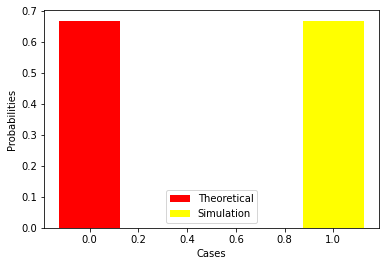
\includegraphics[scale=0.65]{sim_plot.png}
\begin{figure}[h]
\caption*{\textbf{Markov chain diagram}}
\centering
\begin{tikzpicture}
    % Setup the style for the states
        \tikzset{node style/.style={state, 
                                    minimum width=1.2cm,
                                    line width=0.85mm,
                                    fill=gray!20!white}}
        % Draw the states
        \node[node style] at (3, -3)      (bull)     {1};
        \node[node style] at (0, -6)      (bear)     {2};
        \node[node style] at (6, -6) (stagnant) {4};
        \node[node style] at (3, -9)
        (loss) {3};
        % Connect the states with arrows
        \draw[every loop,
              auto=right,
              line width=0.7mm,
              >=latex,
              draw=red,
              fill=red]
            (stagnant)     edge[loop right]            node {1} (stagnant)
            (bull)     edge[bend right=20] node {$\dfrac{1}{2}$} (bear)
            (bear)     edge[bend right=20] node {$\dfrac{1}{2}$} (bull)
            (bull)     edge[bend left=20] node {$\dfrac{1}{2}$} (stagnant)
            (bear) edge[bend right=20]
            node{$\dfrac{1}{2}$} (loss)
            (loss) edge[loop right] node{1} (loss)
            
\end{tikzpicture}
\end{figure}
\end{document}